\documentclass[12pt,a4paper]{article}
%\documentclass{scrartcl}

\usepackage[utf8]{inputenc}
\usepackage[french]{babel}
\usepackage[T1]{fontenc}
\usepackage{graphicx}
\usepackage{fourier}
%\usepackage{lmodern}
\usepackage{helvet}
%\usepackage[scaled]{helvet}
\renewcommand{\familydefault}{\sfdefault}
\usepackage[a4paper, hmargin=113pt, vmargin=111pt]{geometry}
%\usepackage[bindingoffset=5mm]{geometry}
\usepackage{microtype}
\usepackage[hidelinks]{hyperref}
%\usepackage{microtype}%meilleur réglage espaces typo, pb avec les -- dans les tableaux
\usepackage{pdflscape}
\usepackage{longtablex}
\usepackage{tabularx}
\usepackage{multirow}
\usepackage{calc}
\usepackage{wrapfig}
\usepackage{xcolor}
\usepackage{pdfpages}
\usepackage{epigraph}
%\usepackage{scrtime}%heure système
\usepackage{fancyhdr}
\usepackage{titling}


%\usepackage{showframe}
\usepackage{layout}
%\usepackage{lipsum}

\graphicspath{{images/}}
\newlength{\HauteurTexte}
\setlength{\HauteurTexte}{\textheight}

\hypersetup{
    pdftitle={La germination},
    pdfauthor={Pachot, Alexandre},
    pdfsubject={Dossier CRPE 2015},
    pdfkeywords={Germination, PS, MS, maternelle, éducation}
}

\pagestyle{fancy}
%\lhead{}
%\chead{\thetitle}
%\rhead{} 
%\cfoot{\thepage}
\renewcommand{\headrulewidth}{0pt}

%\KOMAoptions{%
%	paper=a4,
%	fontsize=12pt,
%	DIV=calc,
%%	BCOR=5mm,
%%	twoside=on,
%}

\begin{document}
	%\layout{}
	\title{La germination en petite et moyenne section}
\author{Alexandre \textsc{Pachot}}
\date{}
\maketitle
	\begin{flushright}
Toute connaissance est un perpétuel devenir entre un\\
état de moindre connaissance et un état plus efficace.

Jean Bernard \textsc{Makanga}

\emph{Jean Piaget simplement expliqué aux étudiants}
\end{flushright}
	\renewcommand{\contentsname}{Sommaire}
\tableofcontents
	\section{Synthèse des fondements scientifiques}
\marginpar{
\includegraphics[width=35pt]{vignette.png}}
\subsection{La graine}
La graine est la structure qui contient et protège l’embryon végétal issu de la reproduction des plantes à fleurs. Elle est constituée d’un \textbf{embryon}, d’une enveloppe protectrice, le \textbf{tégument}, et d’un ou plusieurs cotylédons. Le \textbf{cotylédon} est la feuille primordiale constitutive de la graine qui contient les réserves nutritives nécessaires au premier développement de la plante. Ces réserves peuvent être riches en glucides (ex. : riz), en lipides (ex. : noix) ou en protides (ex. : arachide). Le nombre de cotylédons varie selon les espèces : un pour le blé et le maïs, deux pour les graines de haricot, le pois et le marronnier, et de dix à douze pour les conifères. Pour certaines graines comme la graine de ricin, les réserves ne sont pas au niveau des cotylédons, mais de l’albumen. La graine est un organe fortement déshydraté, ce qui entraine une vie ralentie et permet de survivre à des conditions extrêmes de température, de longévité et de sècheresse. L’organe transporté se nomme la \textbf{semence}, elle se détache de la plante mère ; cela peut être soit la graine soit le fruit et sa dissémination peut se faire par projection de la plante, par le vent, par l’eau ou par les animaux.

\subsection{La germination}
La germination se produit que si des conditions extérieures (\textbf{humidité}, \textbf{température}, \textbf{oxygène}) sont conjointement présentes. La lumière\footnote{Chez les graines à photosensibilité positive, le tégument contient des phytochromes. Ce sont des photorécepteurs d’une des trois familles de photorécepteurs du monde végétal. Sensibles au rouge (660 nm) et au rouge lointain (730 nm), ils jouent un rôle en stimulant ou inhibant la germination.} influence également la germination des graines \cite[p.~374]{Hopkins2003}. %http://www.botanic06.com/site/EvolVie/stade2.htm
%http://forums.futura-sciences.com/biologie/270616-phytochrome-germination.html
%http://www.ressources-pedagogiques.ups-tlse.fr/physiologie-vegetale/M8G08/CHAPITRE%20IV.pdf
%http://www-ijpb.versailles.inra.fr/fr/bs/equipes/physio-germ/
Tant que les facteurs favorables à la germination ne sont pas réunis, la graine est en état de \textbf{dormance}. Certaines graines ont besoin de passer par une période froide pour pouvoir germer. La germination commence avec l’hydratation de la semence et se finit avec la croissance de la radicule. La jeune plante issue de la germination de la graine se nomme la \textbf{plantule}. Elle est constituée d’une \textbf{radicule} qui deviendra la première racine, d’une \textbf{tigelle} qui deviendra la tige, et des cotylédons.

\subsection{Le développement de l’enfant}
Dans son livre \emph{Jean Piaget simplement expliqué aux étudiants}, Jean Bernard Makanga, psychologue du développement de l’enfant, considère que la période qui va deux à six ans est une des périodes les plus importantes au point de vue intellectuel. Lorsqu’il s’agit de dessiner à partir d’un modèle, l’enfant de trois à six ans reproduit ce qu’il sait déjà faire, avec la signification qu’il attribue au modèle. Il a des difficultés à coordonner les éléments qui composent le dessin, il est au stade du \og \textbf{réalisme manqué} \fg{}. En ce qui concerne la logique, l’enfant ne démontre pas encore ce qu’il dit, c’est le stade de la \og \textbf{pensée intuitive} \fg{} \cite{Makanga2015}.
	\section{Séquence pédagogique}
\subsection{Textes officiels}
Sur la page \og L’enseignement des sciences \fg{}\footnote{\url{http://www.education.gouv.fr/cid54197/l-enseignement-des-sciences.html} (mise à jour en mai~2013)} du site internet du ministère de l’Éducation nationale, de l’Enseignement supérieur et de la Recherche, il est précisé que \og \textbf{Dès l’école maternelle, les enfants sont initiés à la démarche d’investigation} qui développe la curiosité, la créativité, l’esprit critique et l’intérêt pour le progrès scientifique et technique. \fg{}

Dans le programme d’enseignement de l’école maternelle \cite{BO2015} qui rentre en vigueur à la rentrée scolaire~2015, le cinquième et dernier domaine se nomme \og \textbf{Explorer le monde} \fg{} avec pour sous-domaines \og Se repérer dans le temps et l’espace \fg{} et \og Explorer le monde du vivant, des objets et de la matière \fg{}. C’est dans ce deuxième sous-domaine que nous allons nous situer, et plus précisément en \og Découvrir le monde vivant \fg{} où il est précisé que les enfants commencent à comprendre ce qui distingue le vivant du non-vivant et que l’enseignant les conduits à observer les différentes manifestations de la vie végétale. Il est attendu que les enfants sachent, à la fin de l’école maternelle, \textbf{reconnaitre les principales étapes du développement d’un végétal}, dans une situation d’observation du réel ou sur une image.

\subsection{Séquence}
\newcounter{NbSeance}
\newcounter{DureeTotale}
\newcounter{DureeTotaleHeure}
\newcounter{DureeTotaleMinutes}

\makeatletter
\ifx\NbSeancestocke\@undefined\relax\else\setcounter{NbSeance}{\NbSeancestocke}\fi
\ifx\DureeTotalestockee\@undefined\relax\else\setcounter{DureeTotale}{\DureeTotalestockee}\fi
\makeatother

\setcounter{DureeTotaleHeure}{\value{DureeTotale}/60}
\setcounter{DureeTotaleMinutes}{\value{DureeTotale}-\value{DureeTotaleHeure}*60}%

\begin{description}
\item[Titre :] La germination
\item[Niveau :] Petite et moyenne section
\item[Période :] 1 ou 2
\item[Domaine :] Explorer le monde.
\item[Sous-domaine :] Découvrir le monde vivant.
\item[Compétence\footnotemark{} (B.O. 2015)	 :]\footnotetext{Aptitude à mobiliser ses ressources (connaissances, capacités, attitudes) pour accomplir une tâche ou faire face à une situation complexe ou inédite (Socle commun de connaissances, de compétences et de culture, 2015).} Reconnaitre les principales étapes du développement d'un végétal.
\item[Prérequis :] Savoir ce qu’est une plante et un arbre.
\item[Objectif :] Savoir que les graines germent et pas le reste.
\item[Nombre de séances :] \theNbSeance
\item[Durée totale :] 
\ifnum\value{DureeTotaleHeure}=0 %laisser un espace après 0
\theDureeTotaleMinutes{}~min
\else\theDureeTotaleHeure{}~h 
	\ifnum\value{DureeTotaleMinutes}=0 %
	\else\theDureeTotaleMinutes
	\fi
\fi
\end{description}
	\newcommand{\seancei}{Le parc}
\newcommand{\seanceii}{Le tri}
\newcommand{\seanceiii}{Toujours rien ?}
\newcommand{\seanceiv}{Je pense}
\newcommand{\seancev}{Je plante}
\newcommand{\seancevi}{J’observe}
\newcommand{\seancevii}{Je conclus}
\newcommand{\seanceviii}{Dessin du gland}
\newcommand{\seanceix}{Évaluation}
\newcommand{\seancex}{Les bulbes}

\begin{landscape}
%\makeatletter
%\newcommand{\showfontsize}{\f@size{} pt}
%\makeatother
%\showfontsize
%\the\baselineskip
\fontsize{10}{12}\selectfont
\setcounter{NbSeance}{0}
\setcounter{DureeTotale}{0}
\newcommand{\seance}{%
	\stepcounter{NbSeance}%
	{\bf \No \theNbSeance{} : }}
\newcommand{\obj}{%
	{\bf Obj. : }}
\newcommand{\duree}[1]{%
	\addtocounter{DureeTotale}{#1}%
	{#1 min}}

\begin{longtablex}{\HauteurTexte}{%
|>{\raggedright}p{3cm}
|>{\raggedright}X
|>{\raggedright}p{3.7cm}
|>{\raggedright}p{2.4cm}
|>{\raggedright}p{2.8cm}
|>{\centering\arraybackslash}p{1cm}
|}

\hline
\bf \centering\arraybackslash Séance \quad Objectif&
\bf \centering\arraybackslash Déroulement&
\bf \centering\arraybackslash Compétences (B.O.~2015)&
\bf \centering\arraybackslash Savoirs&
\bf \centering\arraybackslash Organisation et matériel&
\bf Durée\tabularnewline
\hline\endhead

%\multicolumn{6}{r}{\dots}
%\endfoot

\hline \hline
\endlastfoot


%%%%%%%%%%%%%
% Séance #1 %
%%%%%%%%%%%%%
% Séance / Objectif
%%%%%%%%%%%%%%%%%%%
\seance \seancei \newline
\obj Ramasser des graines.
&
% Déroulement
%%%%%%%%%%%%%
-- Aller au parc.\newline
-- Ramasser des glands, des marrons, des bouts de branche, des feuilles, des cailloux, \dots\newline
-- Retour à l’école.	
&
% Compétences
%%%%%%%%%%%%%
-- Découvrir un nouveau milieu.\newline
-- Produire des images.
&
% Savoirs
%%%%%%%%%
-- La forme du gland et du marron
&
% Organisation et matériel
%%%%%%%%%%%%%%%%%%%%%%%%%
-- 4~groupes\newline
-- Atsem + 3~parents\newline
-- 1~sac / groupe\newline
-- Appareil photo
&
%Durée
%%%%%%
\duree{40}
\tabularnewline
\hline


%%%%%%%%%%%%%
% Séance #2 %
%%%%%%%%%%%%%
% Séance / Objectif
%%%%%%%%%%%%%%%%%%%
\seance \seanceii \newline
\obj Trier ce qui a été récupéré au parc.
&
% Déroulement
%%%%%%%%%%%%%
-- Mettre ensemble ce qui se ressemble.
&
% Compétences
%%%%%%%%%%%%%
-- Classer des objets en fonction de caractéristiques liées à leur forme.\newline
-- Produire des images.
&
% Savoirs
-- Voc. : pareil
%%%%%%%%%
&
% Organisation et matériel
%%%%%%%%%%%%%%%%%%%%%%%%%
-- Ateliers\newline
-- Ce qui a été récupéré au parc\newline
-- Barquettes\newline
-- Appareil photo
&
%Durée
%%%%%%
\duree{20}
\tabularnewline
\hline


%%%%%%%%%%%%%
% Séance #3 %
%%%%%%%%%%%%%
% Séance / Objectif
%%%%%%%%%%%%%%%%%%%
\seance \seanceiii \newline
\obj Donner l’envie de planter des graines.
&
% Déroulement
%%%%%%%%%%%%%
-- Lecture de l’album \emph{Toujours rien ?} de Christian Voltz.\newline
-- \og Avez-vous envie de planter des graines, comme M. Louis ? \fg{} 
&
% Compétences
%%%%%%%%%%%%%
-- S’exprimer dans un langage syntaxiquement correct et précis. Reformuler pour se faire mieux comprendre.
&
% Savoirs
%%%%%%%%%
-- Lorsqu’on plante une graine, il y a une fleur qui pousse.
&
% Organisation et matériel
%%%%%%%%%%%%%%%%%%%%%%%%%
-- Gr. classe\newline
-- \emph{Toujours rien ?}
&
%Durée
%%%%%%
\duree{20}
\tabularnewline
\hline


%%%%%%%%%%%%%
% Séance #4 %
%%%%%%%%%%%%%
% Séance / Objectif
%%%%%%%%%%%%%%%%%%%
\seance \seanceiv \newline
\obj Formuler des hypothèses.
&
% Déroulement
%%%%%%%%%%%%%
-- Retour sur l’album et sur leur désir de planter des graines.\newline
-- Qu’est-ce qui pousse lorsque je l’enterre ? (\textbf{Je me demande})\newline
-- Dictée à l’enseignant (\textbf{Je pense}).\newline
-- Présenter ce qui a été récupérer au parc ainsi que d’autres objets : haricots, pâtes, billes\dots
&
% Compétences
%%%%%%%%%%%%%
-- Prévoir des conséquences.
&
% Savoirs
%%%%%%%%%
-- Voc. : terre, planter, plante, graine, gland, marron, feuille, tige, bois, caillou, pâtes, haricots, billes
&
% Organisation et matériel
%%%%%%%%%%%%%%%%%%%%%%%%%
-- Gr. classe\newline
-- \emph{Toujours rien ?}\newline
-- Haricots, pâtes
&
%Durée
%%%%%%
\duree{20}
\tabularnewline
\hline


%%%%%%%%%%%%%
% Séance #5 %
%%%%%%%%%%%%%
% Séance / Objectif
%%%%%%%%%%%%%%%%%%%
\seance \seancev \newline
\obj Planter ce qui a été suggéré à la séance précédente.
&
% Déroulement
%%%%%%%%%%%%%
-- Choisir ce qu’on va planter.\newline
-- Coller sur le pot l’étiquette de son prénom et de ce qu’on a choisi de planter.\newline
-- Pot : mettre de la terre, ce qui a été choisi et recouvrir de terre.
&
% Compétences
%%%%%%%%%%%%%
-- Intégrer la chronologie des tâches requises
&
% Savoirs
%%%%%%%%%
-- Voc. : séance précédente + pot, étiquette, cuillère
&
% Organisation et matériel
%%%%%%%%%%%%%%%%%%%%%%%%%
-- Atelier\newline
-- Terre, 1 pot / élève, \og graines \fg{}, étiquette, cuillère
&
%Durée
%%%%%%
\duree{20}
\tabularnewline
\hline


%%%%%%%%%%%%%
% Séance #6 %
%%%%%%%%%%%%%
% Séance / Objectif
%%%%%%%%%%%%%%%%%%%
\seance \seancevi \newline
\obj Observer ce qui a germé ou pas.
&
% Déroulement
%%%%%%%%%%%%%
-- Déterrer les \og graines \fg{}.\newline
-- Définir ce qui a germé ou pas.\newline
-- Dictée à l’enseignant (\textbf{J’observe}).\newline
-- Prendre des photos\newline
-- Replanter les graines
&
% Compétences
%%%%%%%%%%%%%
-- Observer une manifestation de la vie végétale.\newline
-- Produire des images.
&
% Savoirs
%%%%%%%%%
-- Voc. : germer, graine, gland, marron, feuille, tige, bois, caillou
&
% Organisation et matériel
%%%%%%%%%%%%%%%%%%%%%%%%% 
-- Atelier\newline
-- Terre, 1 pot / élève, \og graines \fg{}, étiquettes, cuillères\newline
-- Appareil photo
&
%Durée
%%%%%%
\duree{30}
\tabularnewline
\hline


%%%%%%%%%%%%%
% Séance #7 %
%%%%%%%%%%%%%
% Séance / Objectif
%%%%%%%%%%%%%%%%%%%
\seance \seancevii \newline
\obj Distinguer ce qui germe de ce qui ne germe pas.
&
% Déroulement
%%%%%%%%%%%%%
-- Dire ce qui a germé.\newline
-- Dictée à l’enseignant (\textbf{Je conclus}).\newline
-- Comprendre la notion de ce qui germé de ce qui ne germe pas.\newline
-- Relier la notion du vivant à la germination.
&
% Compétences
%%%%%%%%%%%%%
-- Comprendre ce qui distingue le vivant du non-vivant.
&
% Savoirs
%%%%%%%%%
-- Voc. : germer, gland, tige, cotylédon, racines
&
% Organisation et matériel
%%%%%%%%%%%%%%%%%%%%%%%%%
-- Gr. classe\newline
&
%Durée
%%%%%%
\duree{20}
\tabularnewline
\hline


%%%%%%%%%%%%%
% Séance #8 %
%%%%%%%%%%%%%
% Séance / Objectif
%%%%%%%%%%%%%%%%%%%
\seance \seanceviii \newline
\obj Dessiner un gland germé
&
% Déroulement
%%%%%%%%%%%%%
-- Dessiner un gland germé.
&
% Compétences
%%%%%%%%%%%%%
-- Pratiquer le dessin pour représenter, en étant fidèle au réel.
&
% Savoirs
%%%%%%%%%
-- Voc. :  gland, tige, cotylédon, racines
&
% Organisation et matériel
%%%%%%%%%%%%%%%%%%%%%%%%%
-- Atelier\newline
-- Cahier de sciences
&
%Durée
%%%%%%
\duree{20}
\tabularnewline
\hline


%%%%%%%%%%%%%
% Séance #9 %
%%%%%%%%%%%%%
% Séance / Objectif
%%%%%%%%%%%%%%%%%%%
\seance \seanceix \newline
\obj Distinguer ce qui germe de ce qui ne germe pas.
&
% Déroulement
%%%%%%%%%%%%%
-- Associer des vignettes représentant ce qu’on a planté avec des vignettes représentant la germination et la non-germination.
&
% Compétences
%%%%%%%%%%%%%
-- Reconnaitre une étape du développement d’un végétal.
&
% Savoirs
%%%%%%%%%
-- Ce qu’est une graine.
&
% Organisation et matériel
%%%%%%%%%%%%%%%%%%%%%%%%%
-- Atelier
&
%Durée
%%%%%%
\duree{20}
\tabularnewline
\hline


%%%%%%%%%%%%%%
% Séance #10 %
%%%%%%%%%%%%%%
% Séance / Objectif
%%%%%%%%%%%%%%%%%%%
\seance \seancex \newline
\obj Planter des bulbes dans la cour.
&
% Déroulement
%%%%%%%%%%%%%
-- Présentation du matériel de jardinage.\newline
-- Planter le bulbe
&
% Compétences
%%%%%%%%%%%%%
-- Assurer les soins nécessaires aux plantations\newline
-- Produire des images.
&
% Savoirs
%%%%%%%%%
--  Voc. : bulbe, pelle, râteau, plantoir
&
% Organisation et matériel
%%%%%%%%%%%%%%%%%%%%%%%%%
-- Gr. classe\newline
-- Appareil photo
&
%Durée
%%%%%%
\duree{20}
\tabularnewline
\end{longtablex}

\makeatletter
\immediate\write\@auxout{\gdef\string\NbSeancestocke{\theNbSeance}}
\immediate\write\@auxout{\gdef\string\DureeTotalestockee{\theDureeTotale}}
\makeatother

\end{landscape}
	\begin{landscape}
\subsection{Séance détaillée}
\fontsize{10}{12}\selectfont
\newcounter{CompteurDuree}
\newcounter{noActivite}

\newcommand{\duree}[1]{%
	\addtocounter{CompteurDuree}{#1}%
	#1~min (\theCompteurDuree{}~min)%
	}
\newcommand{\activite}{%
    \stepcounter{noActivite}%
    {\bf\No \thenoActivite{} : }}
    
\setcounter{noActivite}{0}

%\makeatletter
%\ifx\DureeTotale\@undefined\relax\else\setcounter{CompteurDuree}{\DureeTotale}\fi
%\makeatother

\setlength\parindent{0pt}

\begin{tabularx}{\HauteurTexte}{X}
\textbf{Séance \no 4 :}  Que va-t-on planter ?\hfill
%\textbf{Durée}: \theCompteurDuree{} min\hfill
\textbf{Matériel :} \emph{Toujours rien ?}, haricots, pâtes\tabularnewline

\textbf{Compétence (B.O. 2015):} Prévoir des conséquences.\hfill
\textbf{Objectif:} Formuler des hypothèses\tabularnewline

\textbf{Vocabulaire :} terre, planter, plante, graine, gland, marron, feuille, tige, bois, caillou\hfill
\textbf{Organisation}: Groupe classe\tabularnewline
\end{tabularx}

\setcounter{CompteurDuree}{0}

\vspace{-12pt}

\begin{longtablex}{\HauteurTexte}{%
|>{\raggedright}p{2cm}
|>{\raggedright}p{6.1cm}
|>{\raggedright}X
|>{\raggedright}p{2.8cm}
|>{\raggedright}p{2cm}
|>{\centering\arraybackslash}p{1.3cm}
|}

\hline
\bf \centering\arraybackslash Activité&
\bf \centering\arraybackslash Enseignant&
\bf \centering\arraybackslash Consignes&
\bf \centering\arraybackslash Élèves&
\bf \centering\arraybackslash Vocabulaire&
\bf \centering\arraybackslash Durée (Total)
\tabularnewline
\hline\endhead

%\hline
%\endfoot

\hline \hline
\endlastfoot


%%%%%%%%%%%%%%%
% Activité #1 %
%%%%%%%%%%%%%%%
\activite{Retour sur l’album}
&
% Enseignant
%%%%%%%%%%%%%%%%%%%
-- Montrer la première de couverture de l’album.
&
% Consignes
%%%%%%%%%%%%%%%%%%%
-- Quel est le titre ?\newline
-- Que se passe-t-il ?\newline
-- Avez-vous envie de faire comme M. Louis ?
&
% Élèves
%%%%%%%%%%%%%%%%%%%
-- Se rappeler du titre de l’album, raconter l’histoire
&
% Vocabulaire
%%%%%%%%%%%%%%%%%%%
-- trou, terre, graine, tasser, oiseau, fleur
&
% Durée
%%%%%%%%%%%%%%%%%%%
\duree{3}
\tabularnewline
\hline


%%%%%%%%%%%%%%%
% Activité #2 %
%%%%%%%%%%%%%%%
\activite{Je me demande}
&
% Enseignant
%%%%%%%%%%%%%%%%%%%
-- Présenter la trace écrite\newline
-- Compléter la première colonne (Je me demande) avec : \og Qu’est-ce qui pousse lorsque je l’enterre ? \fg{} \newline
&
% Consignes
%%%%%%%%%%%%%%%%%%%
-- Peut-on planter n’importe quoi ?
&
% Élèves
%%%%%%%%%%%%%%%%%%%
-- Faire des propositions de ce qu’on va planter.
&
% Vocabulaire
%%%%%%%%%%%%%%%%%%%
-- graine
&
% Durée
%%%%%%%%%%%%%%%%%%%
\duree{3}
\tabularnewline
\hline


%%%%%%%%%%%%%%%
% Activité #2 %
%%%%%%%%%%%%%%%
\activite{Je pense}
&
% Enseignant
%%%%%%%%%%%%%%%%%%%
-- Demander ce que les élèves veulent planter\newline
-- Noter les propositions au tableau (Je pense).
&
% Consignes
%%%%%%%%%%%%%%%%%%%
-- Qu’allons-nous planter ?
&
% Élèves
%%%%%%%%%%%%%%%%%%%
-- Réfléchir sur ce qu’on peut planter.
&
% Vocabulaire
%%%%%%%%%%%%%%%%%%%
-- planter
&
% Durée
%%%%%%%%%%%%%%%%%%%
\duree{6}
\tabularnewline
\hline


%%%%%%%%%%%%%%%
% Activité #4 %
%%%%%%%%%%%%%%%
\activite{La collecte du parc}
&
% Enseignant
%%%%%%%%%%%%%%%%%%%
-- Présenter ce qui a été récolté au parc et trié par les élèves\newline
-- Noter les propositions au tableau (Je pense).
&
% Consignes
%%%%%%%%%%%%%%%%%%%
-- Parmi tout ce que nous avons récolté au parc, qu’allons-nous planter ?
&
% Élèves
%%%%%%%%%%%%%%%%%%%
-- Faire des propositions de ce qu’on va planter.
&
% Vocabulaire
%%%%%%%%%%%%%%%%%%%
-- gland, marron, feuille, tige, bois, caillou
&
% Durée
%%%%%%%%%%%%%%%%%%%
\duree{4}
\tabularnewline
\hline


%%%%%%%%%%%%%%%
% Activité #5 %
%%%%%%%%%%%%%%%
\activite{Pâtes et haricots}
&
% Enseignant
%%%%%%%%%%%%%%%%%%%
-- Présenter d’autres objets à planter\newline
-- Noter les propositions au tableau (Je pense).
&
% Consignes
%%%%%%%%%%%%%%%%%%%
-- Regarder ce que j’ai trouvé à la maison, il y a des haricots, des pâtes et une bille. Parmi ces objets, que peut-on planter ?
&
% Élèves
%%%%%%%%%%%%%%%%%%%
-- Faire des propositions de ce qu’on va planter.
&
% Vocabulaire
%%%%%%%%%%%%%%%%%%%
-- haricots, pâtes, bille
&
% Durée
%%%%%%%%%%%%%%%%%%%
\duree{4}
\tabularnewline
\end{longtablex}



%\makeatletter
%\immediate\write\@auxout{\gdef\string\DureeTotale{\theCompteurDuree}}
%\makeatother
%\fontsize{12}{14.5}\selectfont
%
%\subsection{Évaluation}
%
%L’évaluation est constituée de vignettes à découper (fig. \ref{bande}) et à coller sur la feuille d’évaluation (fig. \ref{eval}).


\end{landscape}





	\subsection{Traces écrites}
La principale trace écrite consistera à compléter au fur et à mesure des séances le tableau représenté à la figure~\ref{te} qui sera reproduit sur une feuille au format A3.

\newcommand{\echelle}{.985}
\begin{figure}[h!tbp]
\centering
\noindent\fcolorbox{black}{white}{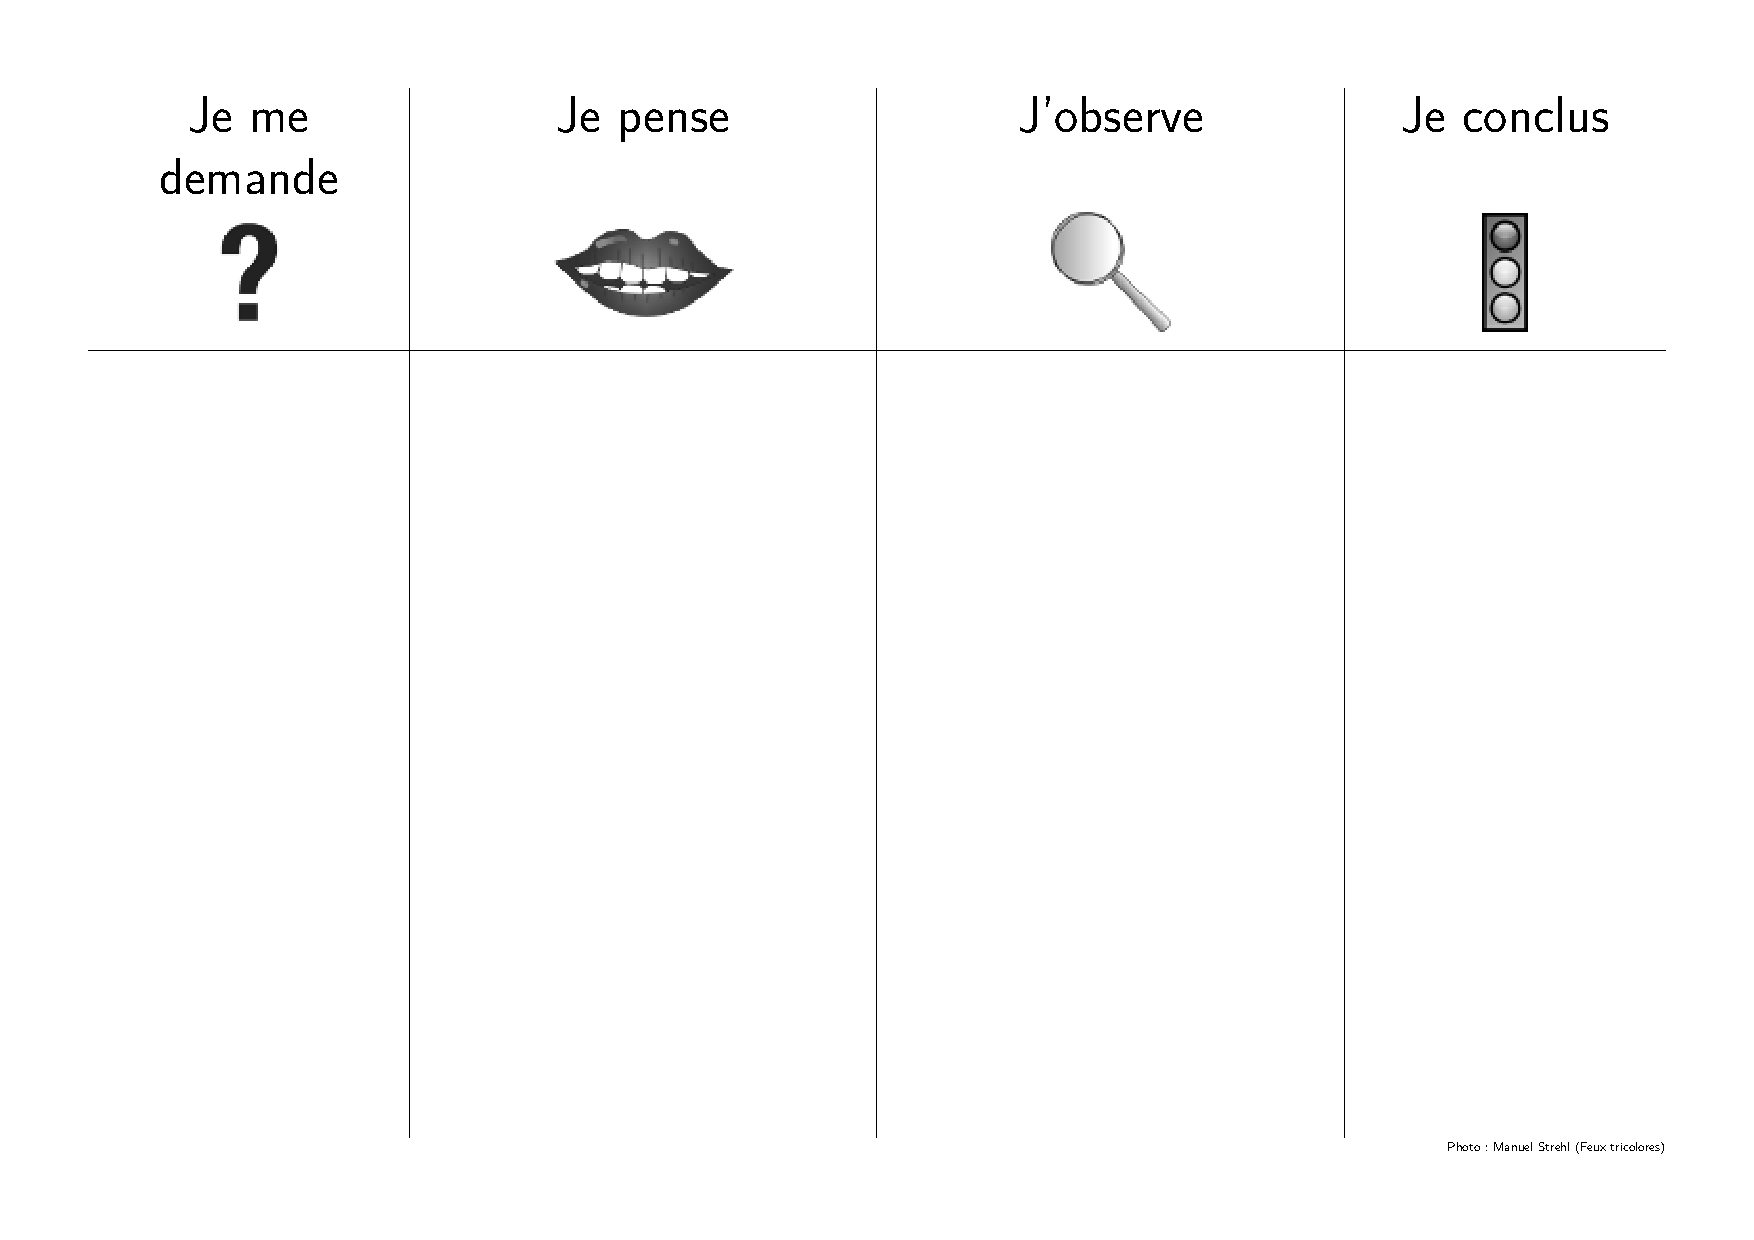
\includegraphics[width=\echelle\textwidth]{tex/TEaffiche.pdf}}
\caption{La démarche d’investigation en maternelle}
\label{te}
\end{figure}

Voici un aperçu des traces écrites.
\begin{description}
\item[Séance 1, \og \seancei \fg{}] Des photos du parc et de ce qu’on y trouve vont être prises par les enfants.
\item[Séance 2, \og \seanceii \fg{}] Des photos sont également prises une fois le tri réalisé. Elles iront enrichir le cahier de vie de la classe ou de l’enfant.
\item[Séance 3, \og \seanceiii \fg{}] Aucune trace écrite.
\item[Séance 4, \og \seanceiv \fg{}] Première et deuxième colonne du tableau : \textit{Je me demande} (Qu’est-ce qui pousse lorsque je l’enterre ?) et \textit{Je pense}.
\item[Séance 5, \og \seancev \fg{}] Pas de trace écrite. Néanmoins, chaque enfant aura un pot, avec l’étiquette de son prénom, ainsi qu’une vignette représentant ce qu’il a mis dans le pot.
\item[Séance 6, \og \seancevi \fg{}] Des photos ainsi que la troisième colonne du tableau : \emph{J’observe}.
\item[Séance 7, \og \seancevii \fg{}] Dernière colonne de tableau : \emph{Je conclus}.
\item[Séance 8, \og \seanceviii \fg{}] Dessin d’un gland germé dans le cahier de science.
\item[Séance 9, \og \seanceix \fg{}] Feuille d’évaluation.
\item[Séance 10, \og \seancex \fg{}] Pas de trace écrite.
\end{description}
	\subsection{Évaluation}
L’évaluation est constituée de vignettes à découper (fig.~\ref{bande}) et à coller sur la feuille d’évaluation (fig.~\ref{eval}, p.~\pageref{eval}). Le critère d’évaluation de la compétence \og Reconnaitre une étape du développement d’un végétal \fg{} est précisé à la table~\ref{criteres}.

\begin{figure}[h!tbp]
\centering
\noindent
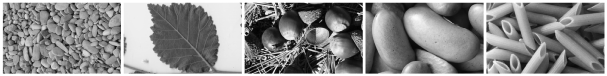
\includegraphics[width=\echelle\textwidth]{bande.png}
\caption{Vignettes à découper}
\label{bande}
\end{figure}

\begin{figure}[h!tbp]
\centering
\noindent
\fcolorbox{black}{white}{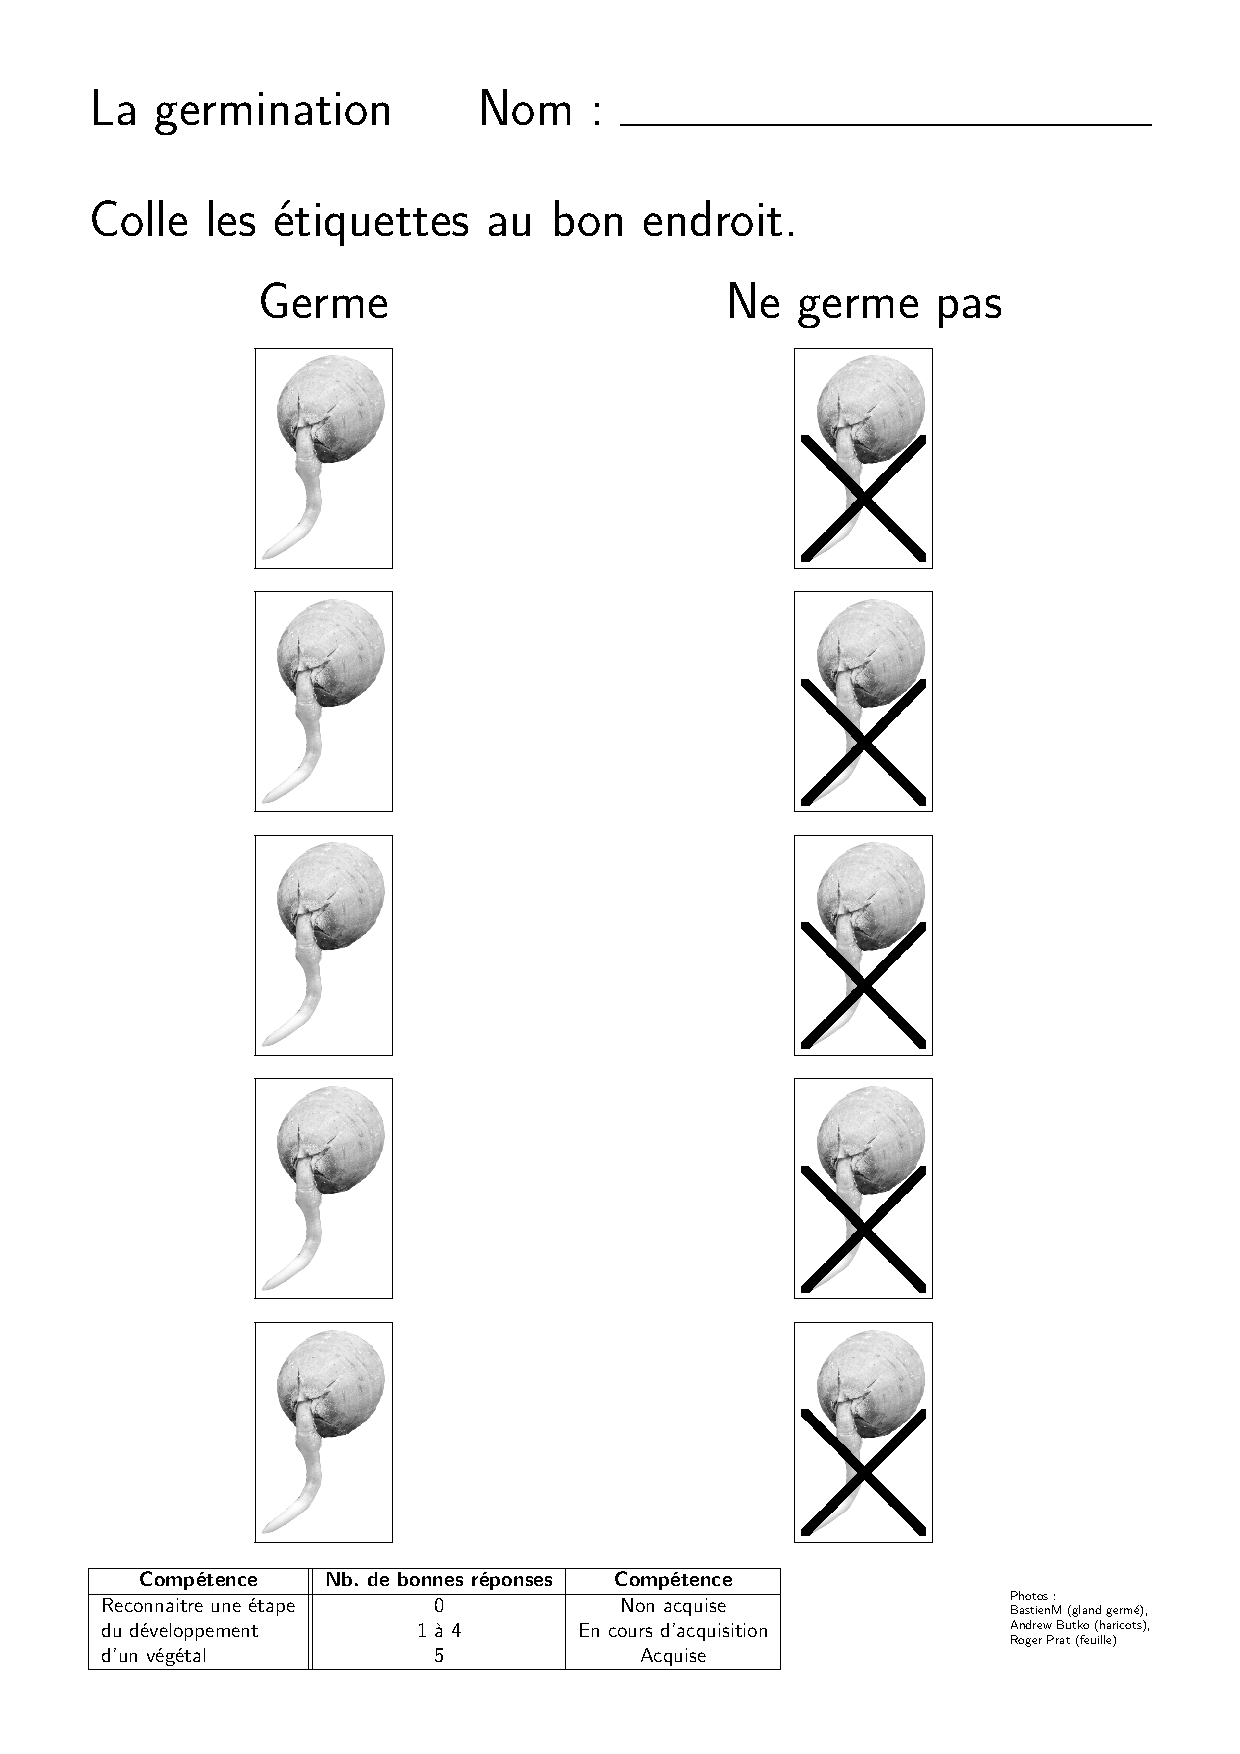
\includegraphics[width=\echelle\textwidth]{tex/eval.pdf}}
\caption{Feuille d’évaluation}
\label{eval}
\end{figure}

\setcounter{table}{0}
%\renewcommand\tablename{\textsc{Tableau}}
\begin{table}[h!tbp]
\centering
\begin{tabular}{|c|c|}
\hline 
\textbf{Nb. de bonnes réponses} & \textbf{Compétence} \\ 
\hline 
0 & Non acquise \\ 
1 à 4 & En cours d’acquisition \\
5 & Acquise \\ 
\hline 
\end{tabular}
\caption{\label{criteres} Critère d’évaluation}
\end{table}

\clearpage
	\bibliographystyle{plain-fr}
\nocite{Lamarque2006}
\bibliography{../commun/ESPE}
%\bibliography{commun/ESPE}
	%\vfill
\subsubsection*{Crédits iconographiques}
Images qui ne sont pas dans le domaine public (mais sous licence CC BY-SA) :
\begin{itemize}
\item Feux tricolores, Manuel Strehl, \url{https://commons.wikimedia.org/wiki/File:Ampel.svg}
\item Feuille d’orme, Roger Prat, \url{https://commons.wikimedia.org/wiki/File:Orme-feuille.jpg}
\item Haricots, Andrew Butko, \url{https://commons.wikimedia.org/wiki/File:Ab_food_19.jpg}
\item Gland germé, BastienM, \url{https://commons.wikimedia.org/wiki/File:Gland_germé_d'un_chêne.jpg}
\end{itemize}

%http://commons.wikimedia.org/wiki/File:Point_d_interrogation.jpg
%http://pixabay.com/fr/bouche-l%C3%A8vres-dent-sourire-256328/
%http://pixabay.com/fr/loupe-verre-bureau-grossissant-23612/

%http://pixabay.com/fr/cailloux-pierre-texture-gris-511932/
%http://commons.wikimedia.org/wiki/File:Orme-feuille.jpg
%http://pixabay.com/fr/noix-gland-noir-ch%C3%AAne-60812/
%https://commons.wikimedia.org/wiki/File:Ab_food_19.jpg
%http://pixabay.com/fr/p%C3%A2tes-pene-pene-rigate-italien-691811/
%http://commons.wikimedia.org/wiki/File:Gland_germ%C3%A9_d%27un_ch%C3%AAne.jpg
	%\begin{center}
\center
\vfill
\aldine
\vfill
Cette œuvre est mise à disposition selon les termes de la licence Creative Commons : attribution, partage dans les mêmes conditions, 4.0, internationale.\quad(CC BY-SA 4.0)\\[1em]


\includegraphics[height=2em]{by-sa}
%
\includegraphics{by-sa}
\vfill

	\def\grabtimezone #1#2#3#4#5#6#7#8#9{\grabtimezoneB}
\def\grabtimezoneB #1#2#3#4#5#6#7{\grabtimezoneC}
\def\grabtimezoneC #1#2'#3'{UTC#1#2\string:#3}
\thispagestyle{empty}
Ce document, composé en \LaTeX{} avec la police de caractères Latin Modern en corps~12, a été compilé le \today{} à \thistime[\ h\ ]
%    UTC+00\string:00.%sharelatex
\expandafter\grabtimezone\pdfcreationdate.
\end{document}

https://books.google.ca/books?id=RHCN1cQwiagC&pg=PA824&dq=germination+dur%C3%A9e+du+jour&hl=fr&sa=X&ei=6q9XVcW7GoimyASH5oCQAQ&ved=0CCkQ6AEwAg#v=onepage&q=germination%20dur%C3%A9e%20du%20jour&f=false
https://books.google.ca/books?id=mT0oLd0L5ykC&pg=PA166&lpg=PA166&dq=graine+dormance+secondaire&source=bl&ots=ccjoZE3nMK&sig=zWr3BehFrZFyowWtuqRPbmBsn1Y&hl=fr&sa=X&ei=ZAhYVbDYG4euyQT6joHoAw&ved=0CDEQ6AEwAw#v=onepage&q=graine%20dormance%20secondaire&f=false
http://www.ia22.ac-rennes.fr/jahia/webdav/site/ia22/shared/maternelle/Groupe%20maternelle/jeux%20symboliques%20Sylvie%20Jouet.pdf
http://www.enfance-dessins-et-personnalites.ch/dessins.html